\chapter{Small World Options}
\label{chap:sw}

In this chapter, we describe how an MDP can be viewed as a graph, and
how Kleinberg's small-world model can be adapted to this setting
(\secref{sec:sw:graph-view}). We then prove that small world options
indeed guarantee a logarithmic bound on the number of decisions taken by
the agent (\secref{sec:sw:theory}). In line with our general theme of
abstraction learning schemes relying only information readily available
to the agent, we describe an efficient algorithm to learn small world
options completely through trajectories taken by the agent
(\secref{sec:sw:algo}). Finally, we evaluate the small world options,
comparing the options against another state of the art technique in
\secref{sec:sw:experiments}.

\section{Graph View of MDPs}
\label{sec:sw:graph-view}

\begin{figure}[th]
    \centering
    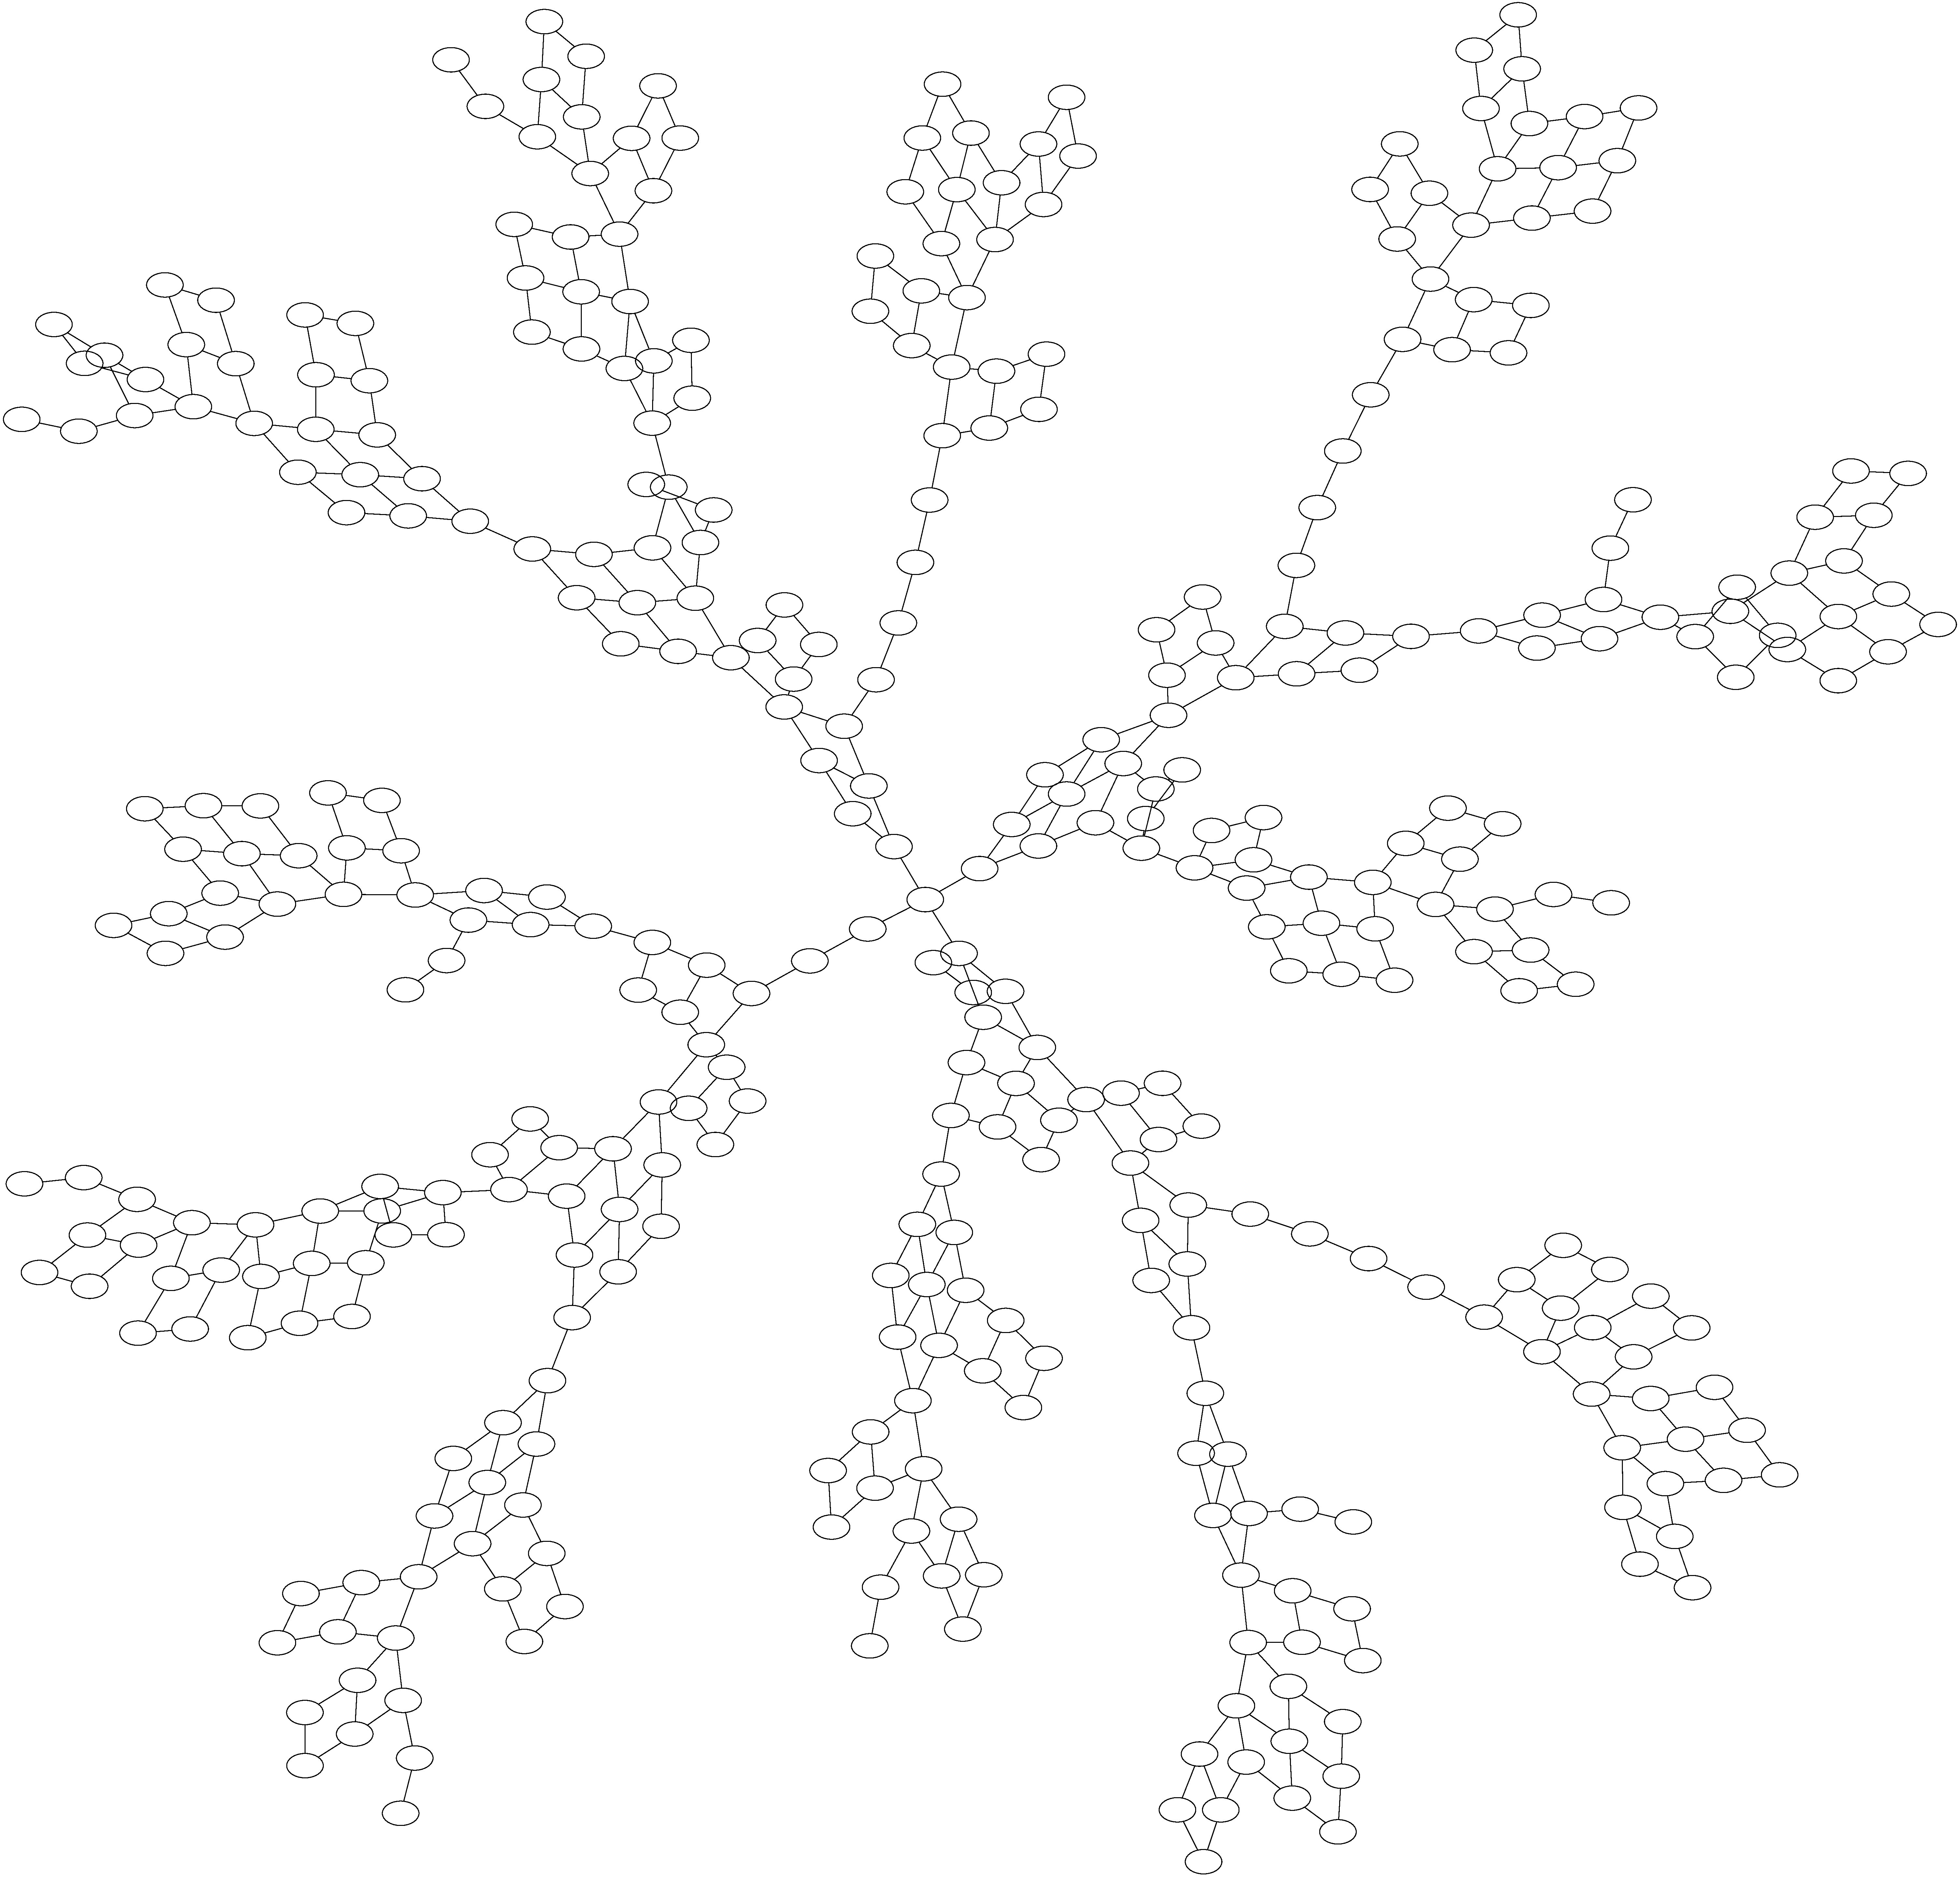
\includegraphics[height=3in]{figures/taxi1}
    \caption{The State Space Graph for Taxi}
    \label{fig:taxi-graph}
\end{figure}

% Graph-based
It is easy to construct a graph $\graph_{\mdp}$ out of the state-space
described by an MDP. The states $\states$ become the nodes of the graph,
and actions $\actions$ become the edges, with the transition
probabilities as weights. Options can be viewed as paths along the
graph. The Taxi domain defined earlier
(\hyperref[example:taxi]{Example~\ref*{example:taxi}}) translates to the
graph shown in \figref{fig:taxi-graph}.

We draw a parallel to the network structure in Kleinberg's small-world
network model (\figref{fig:kleinberg-sw}), by adding a single `path
option' from each state $s$ to another state $s'$, where $s'$ is chosen
with probability $P_r(s,s') \propto \|s-s'\|^{-r}$.  A path option
$o_p(s,s')$ is an option with $\initset = \{s\}$, $\stopcond = \{s'\}$,
and an optimal policy to reach $s'$ for $\pi$.  Intuitively, it is an
option that takes the agent from $s$ to $s'$. In practice, we may
generate path options for only a subset of $|S|$. Note that while this
results in $O(|S|)$ options, only one additional option is available in
any state, and thus the decision-space for the agent is not
significantly larger.

\section{Small World Structure in MDPs}
\label{sec:sw:theory}

Consider an MDP $\mdp_{\klein_r}$ with states connected in
a $r$-dimensional lattice, and noisy navigational actions between
states. We claim that by using {\em robust} path options distributed
according to $P_r$, an $\epsilon$-greedy agent can reach a state of
maximal value using $O(\log(|S|)^2)$ options, using the value function
$\Vf$ as a local property of the state. 

\begin{definition}
    A {\em robust path option} $o(u,v)$, where $u,v \in \states$ is an
    option that takes the agent from $u$ to $v$ `robustly', in the
    sense that in each epoch, the agent moves closer to $v$ with a
    probability $1-\epsilon > \frac{1}{2}$. \footnote{This condition
    is equivalent to saying that the option takes the agent from $u$
    to $v$ in finite time, and hence is not particularly strong.}.
    Note that this $\epsilon$ includes any environmental effects as
    well.
\end{definition}

In order to handle the $\epsilon$-greedy nature of the algorithm, as
well as the approximate-ness in the distance, we will need to extend
Kleinberg's theorem (\thmref{thm:kleinberg-sw}).

\begin{theorem}
  \label{thm:sw}
  Let $f : V \to \Re$ be a function embedded on the graph $\graph(V,E)$,
  such that, $\kappa_1 \|u-v\| - c_1 \le \|f(u) - f(v)\| \le \kappa_2
  \|u - v\| - c_2$, where $0 \le \kappa_1 \le \kappa_2$, and $0 \le c_2
  \le \frac{c_1}{2}$. Let $M_f$ be the global maxima of $f$. Let
  \egreedyalgo be an $\epsilon$-greedy algorithm with respect to $f$,
  i.e.  an algorithm which chooses with probability $1-\epsilon$ to
  transit to the neighbouring state closest to $M_f$, i.e. $N(u)
  = \argmin_v \|f(v) - f(M_f)\|$.
  
  If $\graph(V,E)$ is $r$-dimensional lattice, and contains a long
  distance edge distributed according to $P_r: p(u,v) \propto
  \|u-v\|^{-r}$, then \egreedyalgo takes $O( (\log |V|)^2 )$ steps to
  reach $M_f$.
\end{theorem}
\begin{proof}

This result is a simple extension of Kleinberg's result in
\cite{Kleinberg2000}, and follows the proof presented there, albeit with
the somewhat cleaner notation and formalism of \cite{Martel2004}. We
begin by defining the necessary formalism to present the proof.

\begin{definition}
Let us define $\ball_l(u)$ to be the set of nodes contained within
a ``ball'' of radius $l$ centered at $u$, i.e.  $\ball_l(u) = \{ v \mid
\|u - v\| < l \}$, and $\sball_l(u)$ to be the set of nodes on its
surface, i.e. $\sball_l(u) = \{ v \mid \|u - v\| = l \}$.

Given a function $f:V \to \Re$ embedded on $\graph(V,E)$, we analogously
define $\ballf_l(u) = \{ v \mid |f(u) - f(v)| < l \}$. For notational
convenience, we take $\ballf_l$ to be $\ballf_l(M_f)$.
\end{definition}

The inverse normalised coefficient for $p(u,v)$ is, 
\begin{eqnarray*}
    c_u &=& \sum_{v \ne u} \|u - v\|^{-r} \\
        &=& \sum_{j=1}^{r(n-1)} \sball_j(u) j^{-r}.
\end{eqnarray*}

It can easily be shown that the $\sball_l(u) = \Theta( l^{k-1} )$.
Thus, $c_u$ reduces to a harmonic sum, and is hence equal to $\Theta(
\log n )$. Thus, $p(u,v) = \|u - v\|^{-r} \Theta(\log n)^{-1}$.

\begin{figure}[tbh]
  \centering
    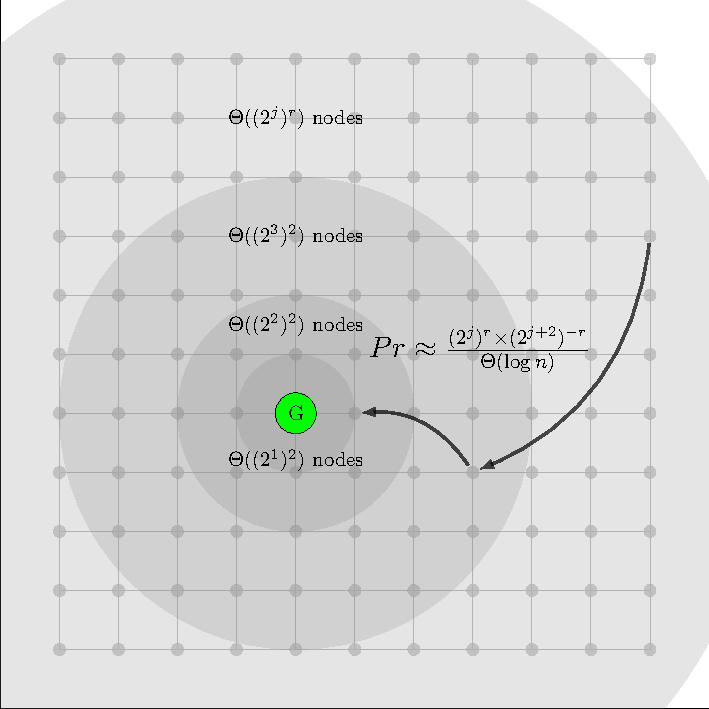
\includegraphics[width=4in]{figures/graph-proof}
    \caption{Exponential Neighbourhoods}
    \label{fig:graph-proof}
\end{figure}

We are now ready to prove that \egreedyalgo takes $O( (\log |V|)^2 )$
decisions. The essence of the proof is summarised in
\figref{fig:graph-proof}. Let a node $u$ be in phase $j$ when $u \in
\ballf_{2^{j+1}} \setminus \ballf_{2^{j}}$. The probability that phase
$j$ will end this step is equal to the probability that $N(u) \in
\ballf_{2^{j}}$. 

The size of $\ballf_{2^{j}}$ is at least $|\ball_{\frac{
2^{j}+c_2}{\kappa_2}}| = \Theta(\frac{2^{j}+c_2}{\kappa_2})$. The
distance between $u$ and a node in $\ballf_{2^{j}}$ is at most
$\frac{2^{j+1} + c_1}{ \kappa_1 } + \frac{2^{j} + c_2}{\kappa_2}
< 2(\frac{2^{j+1} + c_2}{\kappa_2})$. The probability of a link between
these two nodes is at least $(\frac{2^{j+2} + 2 c_1}{\kappa_1})^{-r}
\Theta(\log n)^{-1} $. Thus, 

\begin{eqnarray*}
    P(u, \ballf_{2^{j}} ) &\ge& \frac{(1-\epsilon)}{\Theta( \log n )} (\frac{2^{j}+c_2}{\kappa_2})^{r} \times (\frac{2^{j+2} + 2 c_1}{\kappa_1})^{-r} \\
    &\ge& \frac{(1-\epsilon)}{\Theta( \log n )} \times (\frac{\kappa_1}{4\kappa_2} )^{r} \times ( \frac{ 1 + \frac{c_2}{2^{j}} }{ 1 + \frac{c_1}{2 \times 2^{j}} })^{r}\\
    &\ge& \frac{(1-\epsilon)}{\Theta( \log n )} \times (\frac{\kappa_1}{4\kappa_2} )^{r} \times ( \frac{ 1 + c_2 }{ 1 + \frac{c_1}{2} })^{r} .\\
\end{eqnarray*}

Let number of decisions required to leave phase $j$ be $X_j$. Then, 
\begin{eqnarray*}
    \E[X_j] &\le& \sum_{i=0}^{\infty} (1 - P(u, \ballf_{2^{j}} ))^i \\
            &\le& \frac{1}{P(u, \ballf_{2^{j}} )} \\
            &\le& \Theta( \log n ) \frac{1}{(1-\epsilon)} (\frac{4 \kappa_2}{\kappa_1})^{r} ( \frac{ 1 + \frac{c_1}{2} }{ 1 + c_2 })^{r}\\
            &\le& \Theta( \log n ).
\end{eqnarray*}
Thus, it takes at most $O(\log n)$ decisions to leave phase $j$. By construction, there are at most $\log n$
phases, and thus at most $O((\log n)^2)$ decisions.
\end{proof}

All that remains is to bound the value function, $\Vf$, in terms of the
graph distance to the value maxima. We show this in the following lemma.

\begin{lemma}
    \label{lm:distance}
    Let $o(u,v)$ be the preferred option in state $u$, and let $\|u -
    v\|_V = |\log \Vf(v) - \log \Vf(u)|$. Then, 
    \begin{align*}
        k_1 \|u - v\| - c_1 & \le & \|u - v\|_V & \le & k_2 \|u - v\|, 
    \end{align*}
    \noindent
    where $k_1 = \log \frac{1}{\gamma} $, $k_2 = \log
    \frac{1}{(1-\epsilon)\gamma}$, and $c_1 = \log
    \frac{1}{1-\gamma}$.
\end{lemma}
\begin{proof}
    From the Bellman optimality condition, we get the value of $o(u,v)$ to be,
    \begin{eqnarray*}
        \Qf(u, o(u,v)) &=& \E_{l}[ \gamma^{l} \Vf(v) + \sum_{i=1}^{l} \gamma^{i-1} r_i ],
    \end{eqnarray*}
    \noindent
    where $l$ is the length of the option, and $r_i$ is the reward
    obtained in the $i$-th step of following the option. 
    
    If o(u,v) is the preferred option in state $u$, then $\Vf(u) =
    \Qf(u, o(u,v))$.  Using the property that $0 \le r_i \le 1$,
    \begin{align}
        \E_{l}[ \gamma^{l} \Vf(v) ] &\le& \Vf(u) &\le& \E_{l}[ \gamma^{l} \Vf(v) + \sum_{i=1}^{l} \gamma^{i-1}] \nonumber \\
        \E_{l}[ \gamma^{l} ] \Vf(v) &\le& \Vf(u) &\le& \E_{l}[ \gamma^{l} ] \Vf(v) + \frac{1}{1 - \gamma}. \label{eq:v-bound}
    \end{align}

    $\E_{l}$ is an expectation over the length of the option. Using
    the property that $o(u,v)$ is robust, we move closer to $v$ with
    probability $\epsilonm = 1 - \epsilon$; this is exactly the setting of the
    well-studied gambler's ruin problem, where the gambler begins with
    a budget of $\|u-v\|$, and wins with a probability of $\epsilon$.
    Using a standard result from Feller\cite{Feller1968}, with $m
    = \|u-v\|$, we have,
    \begin{eqnarray*}
        E_l[x^l] = \sum_{l=0}^{\infty} P(L = l) x^{l} &=& \frac{1}{\lambda_1^m( x ) + \lambda_2^m( x )},
    \end{eqnarray*}
    \noindent
    where $\lambda_1(x) = \frac{1 + \sqrt{1 - 4\epsilon\epsilonm
    x^2}}{2\epsilonm x}$, and $\lambda_2(x) = \frac{1 - \sqrt{1
    - 4\epsilonm\epsilon x^2}}{2\epsilonm x}$. When $x \le 1$, 
    \begin{align*}
        \frac{1}{ (\lambda_1( x ) + \lambda_2( x ) )^{m} }  &\le&  E_l[x^l] &\le& \sum_{l=m}^{\infty} P(L = l) x^{l} \\
        \frac{1}{(\frac{2}{2\epsilonm x})^m}  &\le&  E_l[x^l] &\le& \sum_{l=m}^{\infty} P(L = l) x^{m} \\
        (\epsilonm x)^m  &\le&  E_l[x^l] &\le& x^m.
    \end{align*}

    Substituting $x = \gamma$ and $m = \|u - v\|$ into
    \eqnref{eq:v-bound}, we get,
    \begin{align*}
        \E_{l}[ \gamma^{l} ] \Vf(v) &\le& \Vf(u) &\le& \E_{l}[ \gamma^{l} ] \Vf(v) + \frac{1}{1 - \gamma} \\
        (\epsilonm \gamma)^{\|u-v\|} \Vf(v) &\le& \Vf(u) &\le& \gamma^{\|u-v\|} \Vf(v) + \frac{1}{1 - \gamma} \\
        \|u-v\| \log \frac{1}{\gamma} - \log \frac{1}{1-\gamma} &\le& \|u - v\|_V &\le& \|u-v\| \log \frac{1}{\epsilonm \gamma}.
    \end{align*}
\end{proof}

Thus, an $\epsilon$-greedy agent acting with respect to its value
function can reach the maxima of the value function using just $O((\log
|S|)^2)$ decisions. Though this result strictly applies only to the
lattice setting, we observe that many MDPs are composed of lattice-like
regions of local connectivity connected via bottleneck states. The
presence of such bottleneck states would only increase the expected time
by a constant factor. 

\section{Efficiently Constructing Small World Options}
\label{sec:sw:algo}

In \secref{sec:sw:theory}, we remarked that we needed $O(|S|)$ options.
In order to be practical, we require an algorithm to efficiently
generate these options within a budget of training epochs. The proof of
\thmref{thm:sw} provides us with a crucial insight -- our options only
need bring the agent into an exponentially smaller {\em neighbourhood}
of the maximal value state. This suggests that cheaply generated options
may still be acceptable.

The algorithm (\algoref{algo:small-world-experience}) we propose takes
a given MDP $\mdp$, and trains an agent to learn $T$ different tasks
(i.e. different $\rewards$) on it, evenly dividing the epoch budget
amongst them. With each learned task, we certainly will have a good
policy for path options from any state to the state of maximal value,
$M_v$.  However, we observe that will also have a good policy for path
options from $u$ to $v$ is the path is `along the gradient' of $Q$, i.e.
when $V(u) < V(v) < V(M_v)$. Observing that $V(s) \approx \argmax_{v}
Q(s,\pi(s))$, we detail the algorithm to construct many options options
from a single $Q$-value function in \algoref{algo:qoptions}. 

\begin{algorithm}[ht]
  \SetKwInOut{Input}{input}\SetKwInOut{Output}{output}
  \DontPrintSemicolon
  \Input{ $\mdp$, $\Rewards$, $r$, $n$, epochs, $T$ }

  $O \gets \emptyset$ \;
  \For{ $i\gets0$ \KwTo $T$ }{
    $\rewards \sim \Rewards$ \;
    $Q \gets $ Solve $\mdp$ with $\rewards$ using $\frac{\textrm{epochs}}{T}$ epochs \;
    $O' \gets $ QOptions( $Q$, $r$, $\frac{n}{T}$ ) \;
    $O \gets O \cup O'$ \;
  }
  \Return{ A random subset of $n$ options from $O$ }
  \caption{Small World Options from Experience}
  \label{algo:small-world-experience}
\end{algorithm}

\begin{algorithm}[H]
  \SetKwInOut{Input}{input}\SetKwInOut{Output}{output}
  \DontPrintSemicolon
  \Input{ $Q$, $r$, $n$ }
  $O \gets \emptyset$ \;
  $\pi \gets $ greedy policy from $Q$ \;
  \For{ $s$ in $\states$ }{
      Choose an $s'$ according to $P_r$ \;
      \If{ $Q(s', \pi(s')) > Q(s, \pi(s))$ }
      { $O \gets O \cup \tuple{\{s\}, \pi, \{s'\} \cup \{t \mid Q(s',\pi(s')) < Q(t, \pi(t))\} }$ \;
      }{}
  }
  \Return A random subset of $n$ options from $O$
  \caption{{\bf QOptions}: Options from a $Q$-Value Function}
  \label{algo:qoptions}
\end{algorithm}

We note here except for sampling $s'$ from $P_r$, we do not require any
knowledge of the MDP, nor do we need to construct a local model of the
same. In fact, $s'$ can be sampled approximately using the expected path
length instead of the graph distance in $P_r$. As the expected path
length $\E[l]$ is only a constant factor greater than $l$
($\frac{l}{\epsilonm }$), \lmref{lm:distance} continues to hold.

\section{Experimental Results}
\label{sec:sw:experiments}
% Experimental results

We trained MacroQ learning agents on several standard domains, and
measured the cumulative return obtained using the following option
generation schemes: 
\begin{itemize}
   \item \textbf{None}: No options were used.
   \item \textbf{Random}: Options were generated by randomly connecting
     two nodes in the domain (this is equivalent to $P_0$).
   \item \textbf{Betweenness}: As a representative of bottleneck-based
     schemes, options were generated to take any node to a local maxima
     of betweenness centrality, as described in \cite{Simsek2008}. 
   \item \textbf{Small World}: Options were generated randomly
     connecting two nodes of the domain using an inverse square law, as
     described in \secref{sec:sw:theory}.
\end{itemize}

Each experiment, unless mentioned otherwise, was run for $10$ randomly
generated tasks in the domain; each task ran for $40,000$ epochs, and
was averaged over an ensemble of $20$ agents.

\subsection{Optimal Options}
\label{sec:sw:experiments:optimal}
The agents were run on the following three domains using the algorithm
sketched in \secref{sec:sw:theory}:
\begin{itemize}
   \item \textbf{Arbitrary Navigation}: The agent must reach an
     arbitrary goal state in an obstacle-free $x \times y$ grid-world. 
   \item \textbf{Rooms}: The agent must navigate a floor plan with
     4 rooms to reach an arbitrary goal state.
   \item \textbf{Taxi}: This is the domain described in
     \exref{example:taxi}.
\end{itemize}

Optimal policies were given to the options generated according to the
schemes described above. 

\begin{table}
 \centering
 \begin{tabular}{ r | r r r }
  \toprule
             & Arbt. Navi           & Rooms               & Taxi                  \\ 
  \midrule
   None      & -31.82               &  -1.27              & -16.90                \\
   Random    & -31.23               & -10.76              & -18.83                \\
   Betw.     & -18.28               & -8.94               &  {\bf 80.48}          \\
   Sm-W      & {\bf -14.24 [$r=4$]} & {\bf 8.54[$r=2$]}   &   0.66 [$r=0.75$]     \\
  \bottomrule
 \end{tabular}
 \caption{Cumulative Return}
 \label{tbl:optimal-returns}
\end{table}

The results of these experiments are summarised in
Table \autoref{tbl:optimal-returns}. Small world options perform significantly
better than the other schemes in navigation-oriented tasks like Rooms or
Arbitrary Navigation. In the Taxi domain, options generated by the
betweenness scheme outperform the small world options. This is expected
because the goal states in this domain lie at betweenness maxima.

\begin{figure}[tbh]
  \centering
  \subfloat[Rooms: Options learnt]{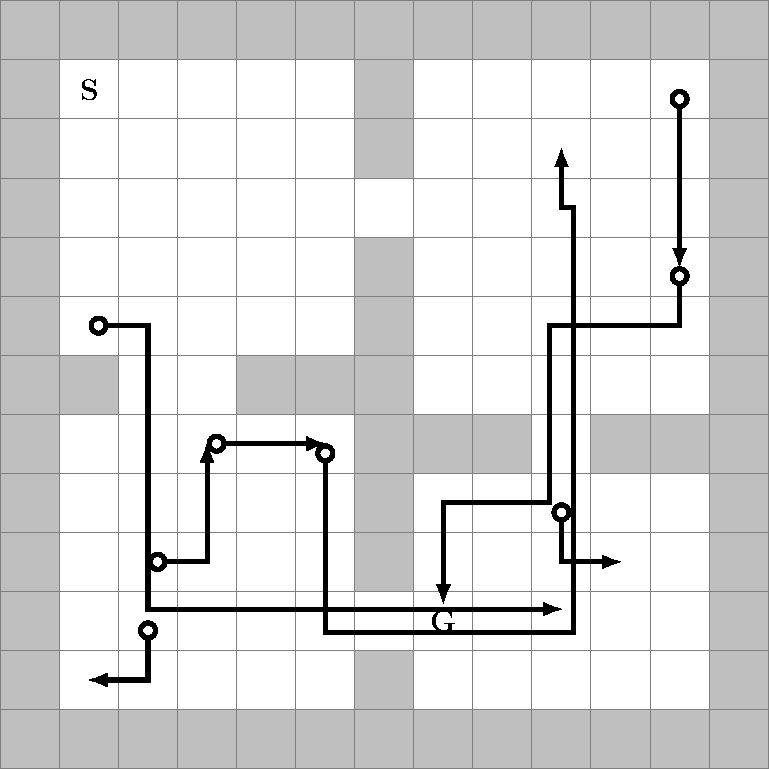
\includegraphics[width=2.4in]{figures/rooms-options}\label{fig:rooms-options}} \hspace{0.25in}
  \subfloat[Rooms: Cumulative Return with 200 options]{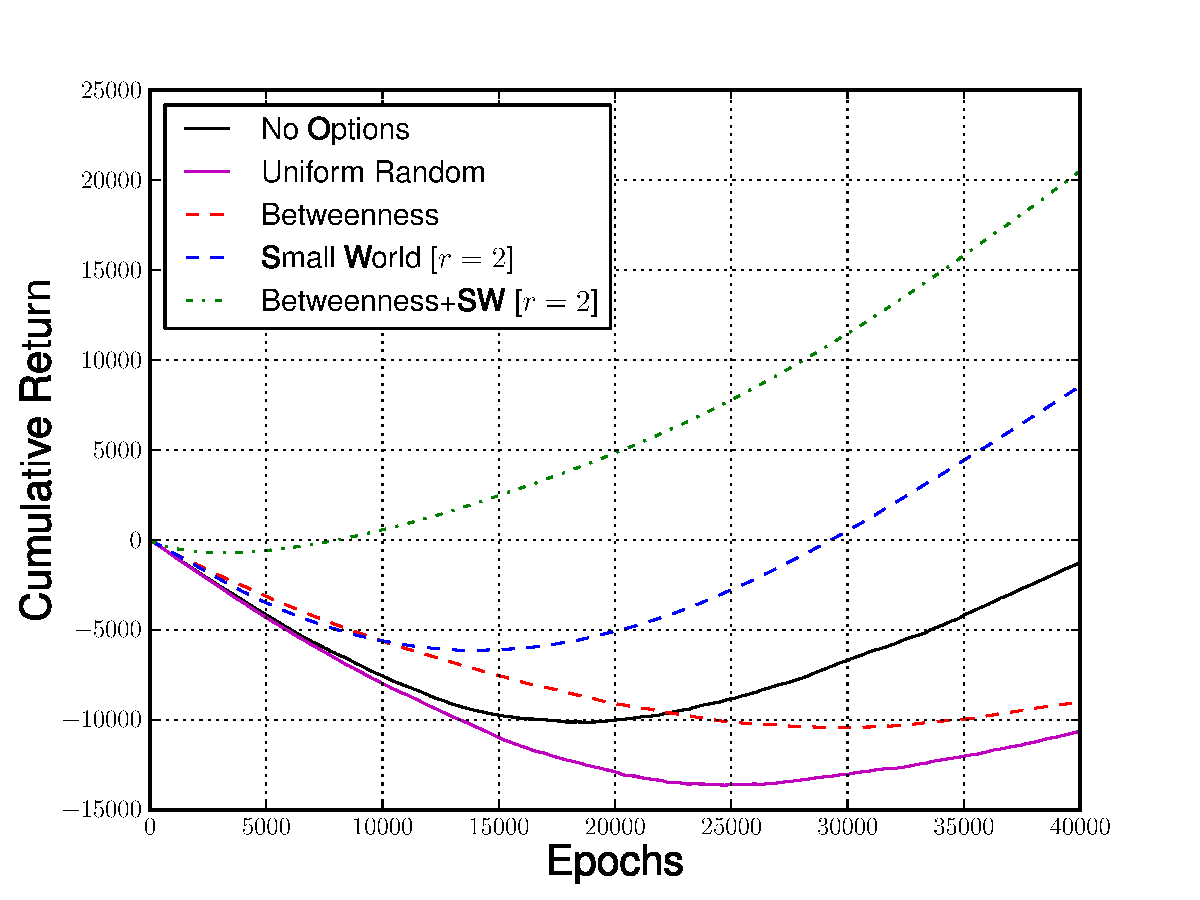
\includegraphics[width=3in]{figures/rooms-return-200}\label{fig:rooms-return}}
\end{figure}

Some of the small world options preferred in Rooms domain are shown in
\figref{fig:rooms-options}. The graph shows several examples of options
that compose together to arrive near the goal state. We have also
plotted the learning behaviour in \figref{fig:rooms-return}. The option
scheme ``Betweenness + SW'' combines options to betweenness maxima with
small world options. Expectedly, it significantly outperforms all other
schemes. The options to betweenness maxima help take the agent between
strongly connected regions, while the small world options help the agent
navigate within the strongly connected region.

\begin{figure}[th]
  \centering
      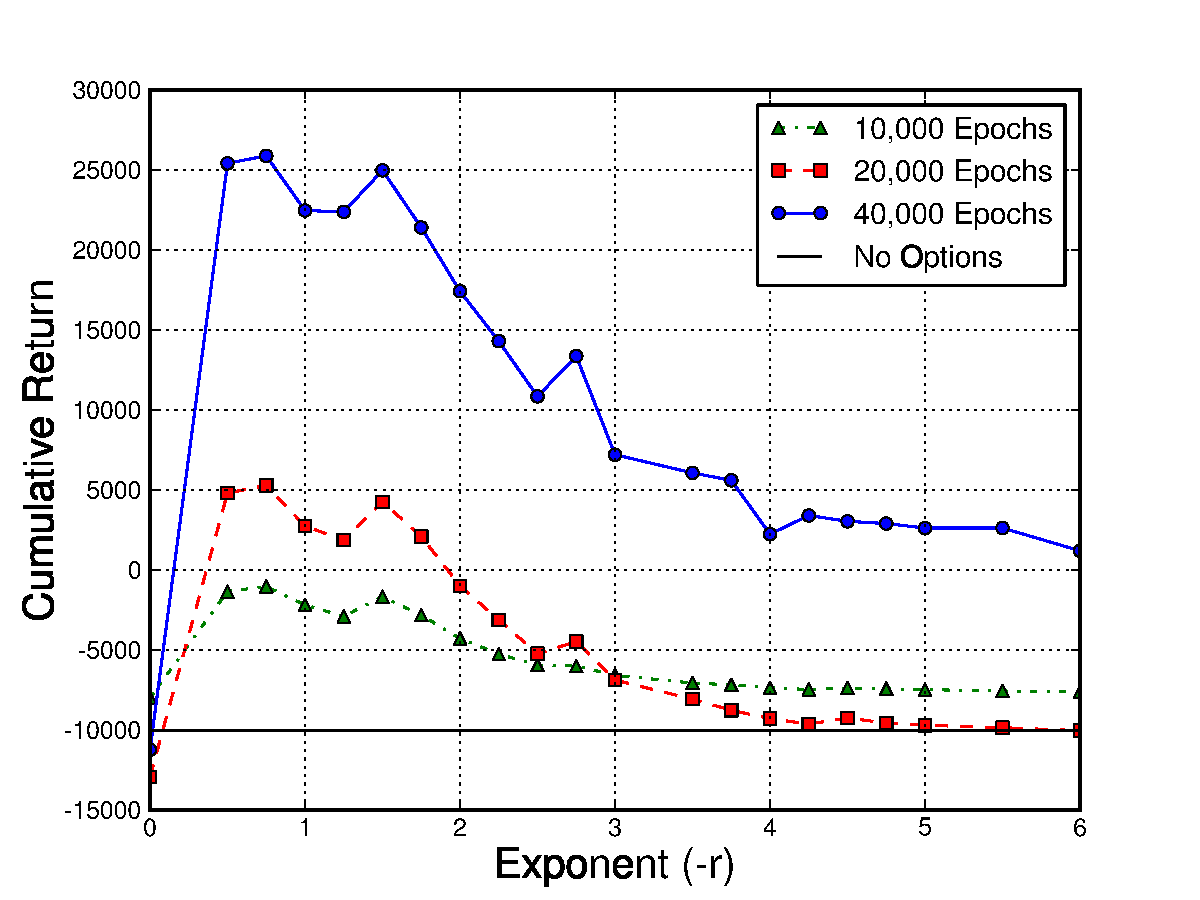
\includegraphics[width=4in]{figures/rooms-exp}
      \caption{Rooms: $r$ vs Cumulative Return}
      \label{fig:rooms-exp}
\end{figure}

\subsection{Sensitivity of $r$}
\label{sec:sw:experiments:sensitivity-r}
\figref{fig:rooms-exp} plots $r$ versus the cumulative return on the
Rooms domain. We do not yet have a clear understanding of how the
exponent $r$ should be chosen. The performance of the agent without
options after $20,000$ epochs is also plotted for reference. There is
a range of $r$ ($\approx 0.75$ to $1.5$) with good performance, after
which the performance steadily drops. This behaviour is easily
explained; as the exponent goes up, the small world options generated
are very short, and do not help the agent get nearer to the maximal
value state. The optimal range of $r$ is slightly counter-intuitive
because the Rooms domain is a two dimensional lattice with some edges
removed. As a consequence of the reduced connectivity, and perhaps due
to stochastic factors, longer range options are preferred.

\begin{figure}[tbh]
  \centering
    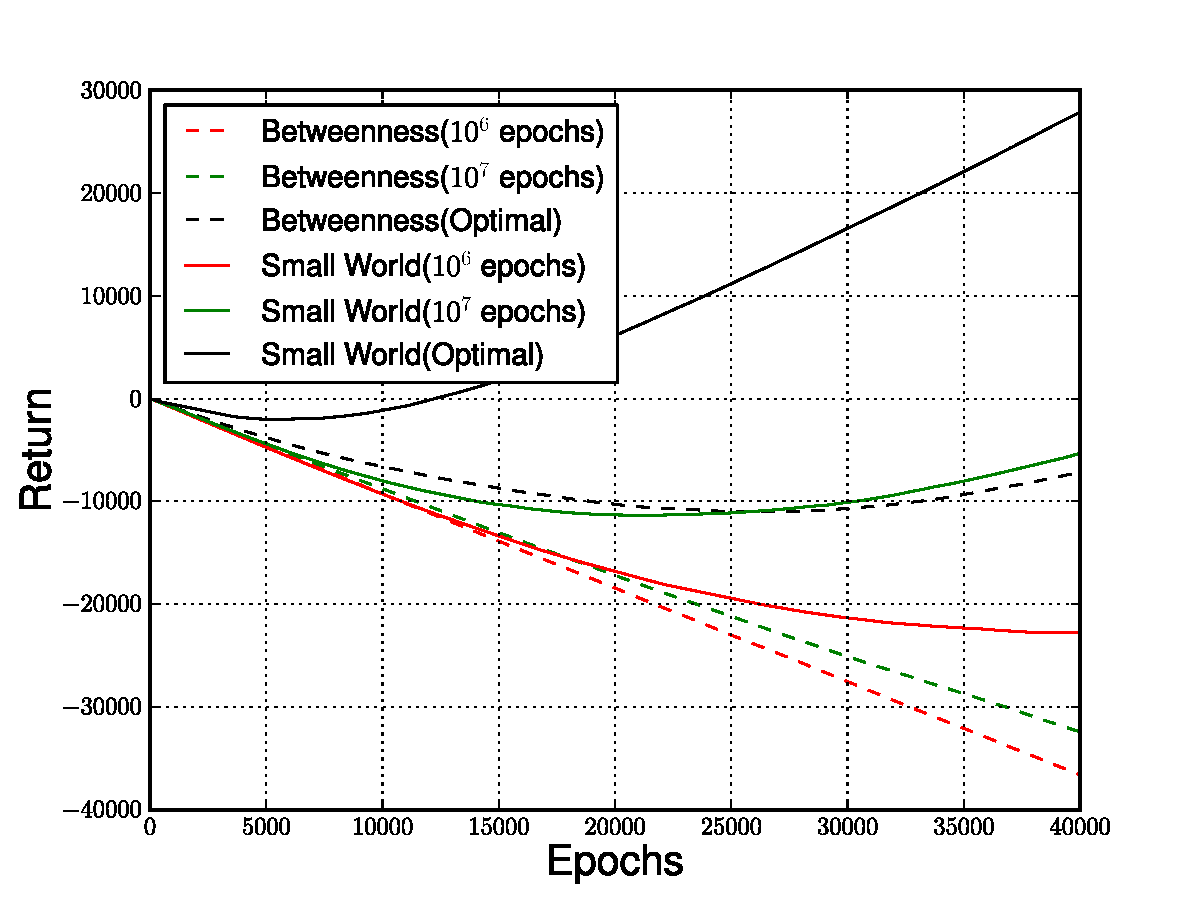
\includegraphics[width=4in]{figures/rooms-learnt-200}
    \caption{Rooms: Options Learnt on a Budget}
    \label{fig:rooms-learnt}
\end{figure}

\subsection{Options Learnt on a Budget}
\label{sec:sw:experiments:budget}
In \secref{sec:sw:algo}, we described an algorithm to construct small
world options efficiently when given a limited number of learning
epochs. We compared the performance of these options with betweenness
options learnt with the same total number of epochs, and have plotted
our results in \figref{fig:rooms-learnt}. Despite using many more
options, the small world options thus created significantly outperform
betweenness options learnt with the same budget, and are even comparable
to the optimal betweenness options.


